\documentclass[oneside,12pt]{report}
\usepackage[utf8]{inputenc}
\usepackage[T1]{fontenc}
\usepackage{graphicx}
\graphicspath{plantillas/}
%\documentclass[oneside,12pt]{report}
\usepackage{fancyhdr}
\usepackage[Lenny]{fncychap}
\usepackage{amsfonts,amssymb}
\usepackage{hyperref}
\usepackage{float,tikz}
\usepackage[footnotesize]{caption}
\usepackage{amsmath,graphicx,multicol,amsthm,latexsym,wasysym,marvosym}
\usepackage{layout}
\usepackage{multirow}
\usepackage{array}
\usepackage{pgfplots}
\usepackage{graphicx} % figuras
\usepackage{subfigure} % subfiguras
%\usepackage{subfig}
\usepackage{subfloat}
\usepackage{setspace}
\usepackage{longtable}
\usepackage{pstricks}
\usepackage{mathtools}
\usepackage{algorithm}
\usepackage{algorithmic}
\usepackage{paralist} 
%\usepackage[print]{pdfscreen}
%\usepackage{enumerate}
\usepackage[spanish]{babel}
\usepackage[utf8]{inputenc}
\usepackage{amsthm}
\usetikzlibrary{shapes,arrows,backgrounds,fit,automata,positioning,shadows}
\usepackage{tocbibind}% incluye la bibliografia al índice
%\usepackage{hyperref}
\voffset-1cm
\hoffset-0.5cm
\parindent 0pt
\parskip .5cm
\setlength{\textwidth}{15.8cm}
\setlength{\textheight}{20.5cm}
%\setlength{\oddsidemargin}{1.5cm}
%\setlength{\evensidemargin}{1.5cm}
\setlength{\marginparwidth}{0cm}
\setlength{\marginparsep}{0cm}
%\usepackage{txfonts}% letra times
%\usepackage[latin1]{inputenc}
\newtheorem{ejem}{Ejemplo}[chapter]
\newtheorem{ejer}{Ejercicio}[chapter]
\newtheorem{prob}{Problema}[chapter]
\voffset-1cm
\hoffset-0.5cm
\parindent 0pt
\parskip .5cm
\setlength{\textwidth}{15.8cm}
\setlength{\textheight}{20.5cm}
%\setlength{\oddsidemargin}{1.5cm}
%\setlength{\evensidemargin}{1.5cm}
\setlength{\marginparwidth}{0cm}
\setlength{\marginparsep}{0cm}
\newcommand{\R}{{\mathbb{R}}}

\renewcommand{\tablename}{\textbf{Tabla}}
%\renewcommand{\qedsymbol}{$\bigstar$}
\renewcommand{\baselinestretch}{1.0}% este para el interlineado
%\renewcommand\thesection{\arabic{section}}
%\phantom{ross} \vspace{1cm}
\pagestyle{fancy} % seleccionamos un estilo
\fancyfoot{} %borra el pie
% Estilo de letra minúscula para los Capítulos
\renewcommand{\chaptermark}[1]{
	\markboth{\chaptername\ \thechapter.\ #1}{}} %
\renewcommand{\sectionmark}[1]{
	\markright{\thesection.\ #1}} %
% Paginación en bold, a la izquiera en pares,
% a la derecha en impares
\fancyhead[LE,RO]{\bfseries\thepage}
% Capítulo a la derecha en pares
\fancyhead[RE]{\bfseries\leftmark}
% Sección a la izquierda en impares
\fancyhead[LO]{\bfseries\rightmark}
\renewcommand{\headrulewidth}{0.3pt} % Width of head rule

%\usepackage[notcite,notref]{showkeys}



\begin{document}
	\shorthandoff{>}\shorthandoff{<}
	\renewcommand{\tablename}{\textbf{Tabla}}
	\thispagestyle{empty}

	\begin{titlepage}
		\begin{center}
			\title
			\date{\textbf{ECUACIONES DIFERENCIALES DE SEGUNDO ORDEN}}\\
			\vspace{4ex}
			%\begin{center}
			\title
			\date{\textsl{VIBRACIONES MECANICAS (AMORTIGUADA, NO AMORTIGUADA,FORZADA Y NO FORZADA) CIRCUITOS ELECTRONICOS}}\normalsize\\ \vspace{8ex}
			\title
			\date{\textbf{PRESENTADO POR:}}\\ \vspace{2ex}
		%\end{center}
			\title
		\date{DIANA MILENA HUERTAS VARGAS}\\ \vspace{5ex}
			\title
		\date{\textbf{PRESENTADO A:}}\\ \vspace{2ex}
		%\end{center}
		\title
		\date{JHONATAN COLLAZOS RAMIREZ}\\ \vspace{3ex}

		\end{center}


\begin{center}
	
\includegraphics[width=0.5\linewidth]{Escudo2}
\end{center}

\begin{center}
		\large{Universidad del Cauca}\\
		\large{Facultad de Ingeniería Civil}\\

\vspace{2ex}	
Agosto 29 de 2022
\end{center}
	\end{titlepage}
\newpage
\chapter{Introducción}

	En el presente proyecto se da a conocer las aplicaciones de las ecuaciones diferenciales de segundo orden;  las que abordaremos directamente en este curso son:  las vibraciones mecánicas y los circuitos eléctricos. Dentro de cada tema se da una breve explicación sobre su definición, la importancia que genera en nuestro entorno, y además se refuerza el tema con un ejemplo explicativo.
	
	Las vibraciones mecánicas son fenómenos presentes en todos los objetos que nos rodea, un claro ejemplo de ello lo podemos encontrar en ventiladores, motores, etc; y los circuitos eléctricos son conjuntos de elementos conectados entre sí por los que puede circular una corriente eléctrica, esto lo podemos aplicar en nuestro diario vivir al encender un bombillo.
	
	\chapter{Preliminares}
En este capitulo trataremos de los conceptos básicos para resolver E.D de segundo orden  homogéneas con  coeficientes constantes, es decir ecuación del tipo
\begin{eqnarray}\label{Edseg}
	ay''+by'+cy=0
\end{eqnarray}
donde, $a, b$ y $c$ son constantes,  para ello,  usando la ecuación auxiliar (Ecuación característica),  se tiene que a resolver la ecuación cuadrática (Raíces del polinomio característico).
\begin{equation}\label{ecuacuad}
	a\lambda^2+b\lambda+c=0
\end{equation}
Esta última ecuación también se le conoce como polinomio característico de la ecuación diferencial (\ref{Edseg}).

Como las dos raíces de (\ref{ecuacuad}) son $m_1 =(- b+\sqrt{b^2- 4ac})/2a$ y $m_2 =(- b-\sqrt{b^2- 4ac})/2a$, habrá tres formas de la solución general de (\ref{Edseg}) que corresponden a los tres casos:
\begin{itemize}
	\item  $m_1$ y $m_2$ reales y distintas $(b^2-4ac>0)$.
	\item $m_1$ y $m_2$ reales e iguales $(b^2-4ac =0)$.
	\item $m_1$ y $m_2$ números conjugados complejos $(b^2- 4ac 
	<0)$.
\end{itemize}
\section{Solución general de una ED de segundo grado}
Analicemos cada uno de estos casos.

\textbf{\textbf{CASO I: RAÍCES REALES Y DISTINTAS}} Bajo la suposición de que la ecuación
auxiliar (\ref{ecuacuad}) tiene dos raíces reales distintas $m_l$ y $m_2$, encontramos dos soluciones de la forma,
$y_1=e^{m_1x}$ y $y_2=e^{m_2x}$. \\
 De ahí que se deduce que la solución
general de (\ref{Edseg}) es:
\begin{equation}
	y=c_1e^{m_1x}+c_2e^{m_2x}
\end{equation}
\textbf{CASO II: RAÍCES REALES REPETIDAS} Cuando $m_1=m_2$, necesariamente se obtiene
sólo una solución exponencial, $y=e^{m_1x}$  y La solución general es entonces es
\begin{equation}
	y=c_1e^{m_1x}+c_2xe^{m_1x}
\end{equation}

\textbf{\textbf{CASO III: RAÍCES COMPLEJAS CONJUGADAS}} Si $m_1$ y $m_2$ son complejas, entonces
se puede escribir $m_1=\alpha+i\beta$ y $m_2=\alpha-i\beta$ donde $\alpha$ y $\beta$	son reales.

Así la solución general esta dada como 
$$y=c_1e^{\alpha x}\cos(\beta x)+c_2e^{\alpha x}\sin(\beta x) $$
\begin{ejem}
	Resolvamos la siguiente ecuación diferencial de segundo orden, la cual es homogénea con coeficientes constantes.
	$$x''-4x'+3x=0$$
	\begin{itemize}
		\item Ecuación característica( Ecuación cuadrática de grado 2 asociada a la ED )
		$$\lambda^2-4\lambda+3=0$$
		el cual tiene la siguientes soluciones $\lambda_1=1$ y $\lambda_2=3$
		\item  Solución general( Se da aparir de las raíces del polinomio)
		$$x(t)=C_1e^{t}+C_2e^{3t}$$
	\end{itemize}
\end{ejem}
	
\section{Vibraciones mecánicas:}	


Las vibraciones mecánicas son un fenómeno presente en todos los objetos que nos rodean y forman parte de nuestro día a día. Por ejemplo, objetos como ventiladores, motores, altavoces, etc.
Un movimiento vibratorio es la variación de configuración de un sistema, en relación al tiempo y en torno a una posición de equilibrio estable. Se caracteriza por ser periódico; por ejemplo, el movimiento armónico simple.
Los sistemas mecánicos responden variando su estado de equilibrio al ser sometidos a la acción de fuerzas variables respecto al tiempo. En consecuencia, presentan cambios de configuración al perturbar su funcionamiento normal. Por tal motivo, el mantenimiento predictivo se interesa por medir las vibraciones de un sistema para determinar sus posibles fallas y atacarlas antes de que sucedan.\\

	
	
	
\textbf{Vibraciones libres Amortiguadas:}\\
	
	
	Los sistemas reales no se mantienen indefinidamente en vibración, ya que siempre hay rozamientos que hacen que pierdan energía hasta que se paran.
	
	De entre los tipos de fuerzas de rozamiento que puede haber, vamos a considerar únicamente el rozamiento fluido o amortiguamiento viscoso, que tiene lugar cuando un cuerpo se mueve dentro de un fluido.
	Este tipo de rozamiento puede ser de origen natural e inevitable como los debidos movimientos en el aire o en agua, o bien puede ser buscado a propósito para eliminar vibraciones indeseadas
	
	Nos limitaremos a amortiguadores lineales: la fuerza de amortiguación se opone a la velocidad y es directamente proporcional al módulo de la velocidad con que se extiende o comprime el amortiguador.
	
	\begin{center}
		\begin{tabular}{rcc}
	
			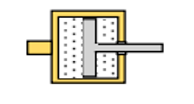
\includegraphics[width=0.4\linewidth]{imagen1}
		
	&&
	\end{tabular}	\begin{tabular}{rcc}
		&&\\[0.5cm]
			&&\\
	&&{\LARGE $\vec{F}=-c\vec{v}$},\vspace{2cm}
\end{tabular}
	\end{center}
	donde,	c:\textbf{ constante de amortiguamiento viscoso} $\left( unidades\hspace{0.2cm} S.I.\hspace{0.2cm} (\frac{N*s}{m})\right) $
\subsection{Aplicación}
\begin{center}
	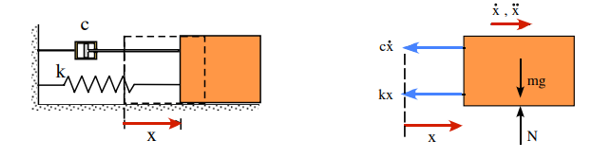
\includegraphics[width=0.7\linewidth]{imagen2}
\end{center}

\textbf{\begin{center}
		SEGUNDA LEY DE NEWTON
\end{center}}
	\begin{equation}
		\sum F_{x}=ma_{x},\hspace{1cm}-kx'(t)-cx(t)=mx''(t)
	\end{equation}
El modelo que describe la segunda ley de Newton a partir de la gráfica anterior es:
\begin{equation}\label{Ecu}
	mx''(t)+kx'(t)+cx(t)=0
\end{equation} 
la cual es una ecuación 	\textbf{\textit{ Diferencial del movimiento: (de segundo orden con coeficientes constantes)}}

El polinomio característico asociado a la ecuación (\ref{Ecu}) es:
\begin{equation}
	\lambda^2+c\lambda+k=0
\end{equation}
Luego, las raíces del anterior polinomio son de la forma: 
\begin{equation}
	\lambda_{1,2}=\frac{-c\pm\sqrt{c^2-4\lambda k}}{2m}
\end{equation}
Vamos a escribir estas raíces en función de las variables:

\begin{equation}
	\omega_{n}=\sqrt{\frac{k}{m}}\longrightarrow \textit{Pulsación natural del sistema}
\end{equation}

\begin{equation}
	\varsigma=\frac{c}{2\sqrt{mk}}=\frac{c}{2m\omega_n}\longrightarrow \textit{o razón de amortiguamineto (adimensional)}
\end{equation}
Por tanto, las raíces las podemos reescribir de la siguiente manera:
\begin{equation}\label{Amortiguamiento}
	\lambda_{1,2}=-\varsigma \omega_n \pm\omega_n\sqrt{\varsigma^2-1}	
\end{equation}
y la solución a la ED es:
$$x(t)=c_1e^{\lambda_1 t}+c_2e^{\lambda_2 t}$$
Observemos que en la ecuación (\ref{Amortiguamiento}) se tiene que:


El valor de $c$ tal que la raíz es cero se llama coeficiente de amortiguamiento crítico, $c_r$ :
\begin{equation}
	c_r=2m\omega_n=2\sqrt{mk}
\end{equation}

\section{Vibraciones no amortiguadas}
Para estudiar las vibraciones libres de un sistema de un grado de libertad, analizamos el modelo matemático más simple formado por un resorte sin masa de constante elástica $k$ y una masa $m $ proveniente del peso puntual $W$ aplicado en uno de sus extremos, según se muestra en la figura al que llamamos sistema masa-resorte $(mk)$, donde m puede solamente moverse según el eje vertical.
\begin{center}
	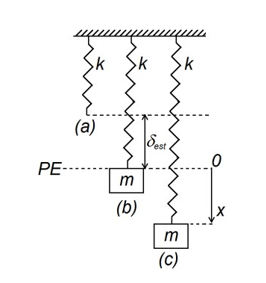
\includegraphics[width=0.4\linewidth]{imagen10}
	\end{center}

Cuando el peso $W$ se cuelga del resorte, éste se estira un valor $\delta_{est}$, llamando deflexión estática o alargamiento estático, hasta alcanzar la posición de equilibrio PE. En esta posición, el efecto de la gravedad sobre m se equilibra con la fuerza elástica reactiva del resorte y se cumple:
\begin{equation}
	k\delta_{est}=W=mg
\end{equation}

(Relación que define la posición de equilibrio PE)


Si a partir de esta posición la masa $m$ es desplazada una distancia $x$, y luego se deja la única fuerza que actúa sobre $m$ es la reacción del resorte y se inicia un movimiento vibratorio gobernado por:

\textbf{El modelo que describe la segunda ley de Newton a partir de la gráfica anterior es:}
\begin{equation}
	\sum F=mx''(t)
\end{equation}
Cuya aplicación es:

\begin{equation}\label{Ecu2}
	W-k(x+\delta_{est})=mx''(t)
\end{equation}
\begin{center}
	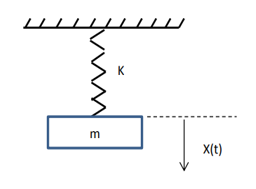
\includegraphics[width=0.6\linewidth]{imagen9}
\end{center}
Teniendo en cuenta la relación que define la posición de equilibrio PE resulta:
\begin{equation}
	mx''+kx=0
	\end{equation}
Si dividimos la anterior  ecuación entre $m$, se tiene que:
\begin{equation}
	x''+\frac{k}{m}x=0
\end{equation}
Donde se definen el siguiente parámetro:
\begin{equation}
	\frac{k}{m}=w_0^{2}=\frac{g}{\delta_{est}}
\end{equation}
Es decir, \begin{equation}
	x''+w_0^{2}x=0
\end{equation}
El parámetro $w_0=\sqrt{\frac{k}{m}}$ Se le conoce como Pulsación natural del sistema.


La solución general de esta ecuación diferencial es:
\begin{equation}
	x=A.sen(w_0.t)+B.cos(w_0.t)
\end{equation}

Donde A y B son constantes que se determinan de acuerdo con las condiciones
iniciales que son, generalmente:

$$t=0\longrightarrow{x}=x_0$$

$$t=0\longrightarrow{x'}=x'_0$$
\section{Vibraciones mecanicas Forzadas}
\begin{center}
	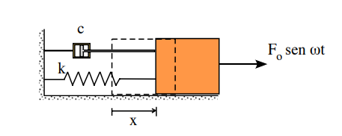
\includegraphics[width=0.7\linewidth]{imagen8}
\end{center}

Se llama así cuando hay una fuerza periódica aplicada al sistema o una perturbación periódica de alguna distancia
\begin{center}
	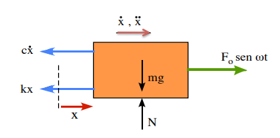
\includegraphics{imagen16}
\end{center}
\begin{equation}
	mx+cx''+kx=F_0sen (\omega t)
\end{equation}

La solución general es:
\begin{equation}
   x(t)=x_h+x_p
\end{equation}

Donde:  
\begin{center}	
\begin{tabular}{rcl}
 $x_h$&$\longrightarrow$& \textbf{Solución general a la ecuación diferencial homogénea}.\\[0.5cm]
$x_p$&$\longrightarrow$ &\textbf{Solución particular de la ecuación diferencial  homogénea}.
\end{tabular}
\end{center}


$x_h$ sería la solución del movimiento libre amortiguado y en cualquier caso representaría un movimiento transitorio que desaparecería al cabo de un tiempo.

Una solución particular en cambio es la vibración estacionaria:

\begin{equation}
	x_p=x_0sen(\omega -\varphi)
\end{equation}
Sustituyendo en la ec. diferencial se obtiene que es solución si:

\begin{equation}
	x_0=\frac{F_0}{\sqrt{(k-m\omega^{2})^{2}+c \omega^{2}}}\hspace{1cm}\tan(\varphi)=\frac{c \omega}{k-\omega^{2}}
\end{equation}

Teniendo en cuenta que:
La frecuencia natural de la vibración libre
$\omega_n= \sqrt{\frac{k}{m}}$

Y el coeficiente de amortiguamiento critico es:

$c_r=2m (\omega_n)$, además 
\begin{equation}
	x_0=\frac{F_0}{K}\sqrt{1-\left( \frac{\omega}{(\omega_n^{2})^{2}+[2(\frac{c}{c_r})(\frac{\omega}{\omega_n})]^{2}}\right) }
\end{equation}
Amplitud de la vibración estacionaria
\begin{equation}
	\tan \varphi=\frac{2(\frac{c}{c_r})(\frac{\omega}{\omega_n})}{1-\left( \frac{\omega}{\omega_n^{2}}\right) }
\end{equation}
Desfase entre la vibración estacionaria y la libre
amortiguada

Siendo $\frac{c}{c_r}$ el factor de amortiguamiento, $\frac{\omega}{\omega_n}$ la razón entre la frecuencia de la fuerza aplicada y la natural del oscilador


Como se puede ver de la expresión de la amplitud, en ausencia de amortiguación (c=0),
si la frecuencia angular de la fuerza aplicada coincide con la natural, la amplitud se
hace infinita. Se dice entonces que hay resonancia

\begin{center}
	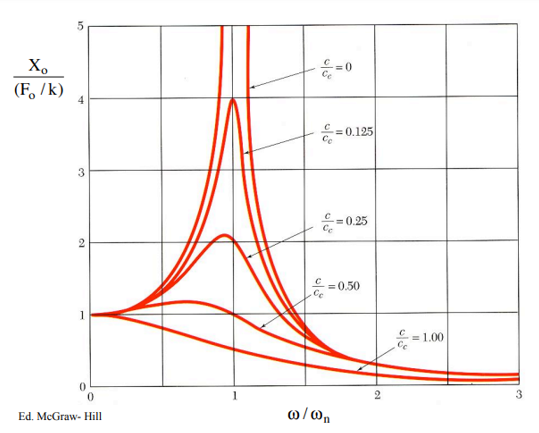
\includegraphics[width=0.8\linewidth]{imagen6}
\end{center}
Una vibración forzada puede provenir del exterior (por ejemplo, un suelo que se mueva
como ocurre en los terremotos) o interior como ocurre cuando en una máquina hay una
rotación descompensada.
Desequilibrio de una pieza giratoria de una máquina:

\begin{center}
	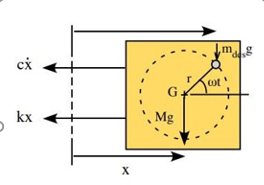
\includegraphics[width=0.5\linewidth]{imagen5}
\end{center}

\begin{equation}
	-cx'-kx=M''+m_{des} \frac{d^{2}(x+r\cos (\omega t))}{dt^{2}}
\end{equation}
	\begin{equation}
			(M+m_{des})x''+cx'+kx=m_{des}r\omega ^{2} \cos\omega t
	\end{equation}
Es la misma ecuación forzada que hemos visto antes con:

$$F_0=m_{des}r\omega ^{2}$$
y
$$m=M+m_{des}$$
\section{Vibraciones Mecánicas no forzadas}
Bloque que cuelga de un resorte de constante elástica k:

\begin{center}
	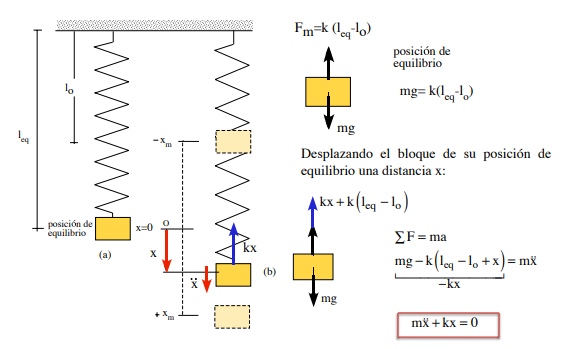
\includegraphics[width=0.8\linewidth]{Captura}
\end{center}

ED de 2º orden con coeficientes constantes:

\begin{equation}
	mx''+kx=0
\end{equation}

La solución es una combinación de exponenciales
\begin{equation}
	x=C_1e^{\lambda_1 t}+C_2e^{\lambda_2 t}
\end{equation}
Para mayor claridad aquí damos el paso a paso de la solución de un ED de segundo orden, la cual es el modelo de un problema físico, para ello:

Siendo $\lambda_1$ y $\lambda_2$, las raíces del polinomio característico

El polinomio característico es el obtenido sustituyendo en la ED

\begin{center}
	$x''\longrightarrow \lambda^{2}$

$x\longrightarrow \lambda$

$x\longrightarrow 1$

\end{center}
En nuestro caso:
\begin{equation}
	m\lambda^{2}+k=0\longrightarrow\lambda^{2}=-\frac{k}{m}\longrightarrow\lambda=\pm i \sqrt{\frac{k}{m}}
\end{equation}
La definición para esta ecuación se tiene que:
 
 \begin{equation}
 	\omega_{n}=\sqrt{\frac{k}{m}}
 \end{equation}

\begin{equation}
x=A sen(\omega_n t)+B\cos(\omega_n t)
\end{equation}
 	Derivando respecto al t:
 \begin{equation}
 	v=x¨=A\omega_n \cos(\omega_n t)-B\omega_n sen(\omega_n t)
 \end{equation}
\begin{equation}
	a=x¨=-A\omega_n^{2} sen(\omega_n t)-B\omega_n^{2} \cos(\omega_n t)=-\omega_n^{2}x
\end{equation}
A y B son constantes a determinar a partir de las condiciones iniciales del problema, otra forma de expresar la solucion es:
\begin{equation}
	x=x_msen(\omega_n t+\varphi)
\end{equation}
\begin{center}
	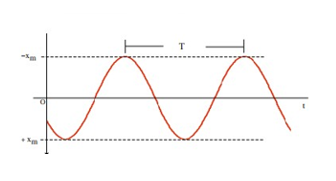
\includegraphics[width=0.7\linewidth]{imagen4}
\end{center}
$$A=x_m cos(\varphi)$$
$$B=x_m sen(\varphi)$$
$\tan(\varphi)=\frac{B}{A}$

$x_m$=\textbf{Amplitud o valor máximo}

$\omega_n$=\textbf{Frecuencia angular o pulsacion natural de la vibracion (rad/s)}\\
$\varphi$= \textbf{Ángulo de fase o desface}\\

$T:$ \textbf{es el periodo o tiempo en que hace una oscilacion completa}

$T=\frac{2\pi}{\omega}$

Frecuencia, $f$=es el número de oscilaciones por unidad de tiempo.

$f=\frac{1}{T}$  (UNIDAD SI:Hz)
\section{Circuitos de segundo orden}

Se caracterizan por una ecuación diferencial de segundo orden, consta de resistores y el equivalente de dos elementos de almacenamiento de energía.

Este análisis es similar al que se realiza con los de primer orden. Primero se consideran circuitos excitados por las condiciones iniciales de los elementos de almacenamiento. Aunque estos circuitos pueden contener fuentes dependientes, están libres de fuentes independientes. Como es de esperar estos circuitos darán respuestas naturales. Después se tratarán circuitos excitados por fuentes independientes, estos circuitos darán tanto la respuesta transitoria como la respuesta en estado estable.

\begin{center}
	\textbf{DETERMINACION DE VALORES INICIALES Y FINALES}
\end{center}
Se debe manejar la polaridad de la tensión v(t) en el capacitor y la dirección de la corriente i(t) a través del inductor. Debemos tener en cuenta que v e i se definen estrictamente de acuerdo con la convención pasiva de los signos. Se deben tener en cuenta como está definida las variables y aplicarlas en secuencias.
También se debe tener presente que la tensión del capacitor siempre es continua de modo que:

$$v(0^{+})=v(0^{-})$$

Y que la corriente del inductor siempre es continua, de modo que:

$$i(0^{+})=i(0^{-})$$ 

Donde $t=0^{-}$ denota el momento justo antes de un evento de conmutación y $t=0^{+}$ es el momento justo después del evento de conmutación, suponiendo que este tiene lugar en $t=0$.
Así para poder determinar los elementos iniciales se deben enfocar en las variables que no pueden cambiar abruptamente. La tensión del capacitor y la corriente del inductor, a continuación, veremos un ejemplo de lo antes mencionado:

El interruptor de la siguiente figura ha estado cerrado mucho tiempo, se abre en  $t=0$, halle $i(0^{+} )$

$v(0^{+})$, $\frac{d_i(0^{+})}{dt}$ , $\frac{d_v(0^{+})}{dt}$, $i(\infty)$, $v(\infty)$
\begin{center}
	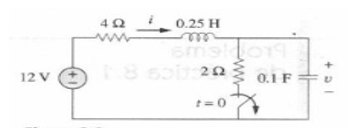
\includegraphics[width=0.7\linewidth]{circuitoejer}
\end{center}
Solucion:

a)	Si el interruptor está cerrado mucho tiempo antes de $t=0$, esto significa que el circuito ha llegado al estado estable de cd en $t=0$, o estado estable de cd, el inductor actúa como un corto circuito, mientras que el capacitor lo hace como un circuito abierto, así que se tienen el circuito de la siguiente manera en t=0. Por tanto

\begin{equation}
	i(0^{-})=\frac{12}{4+2}=2A
\end{equation}
por otro lado,
\begin{equation}
	v(0^{-})=4v
\end{equation}
\begin{center}
	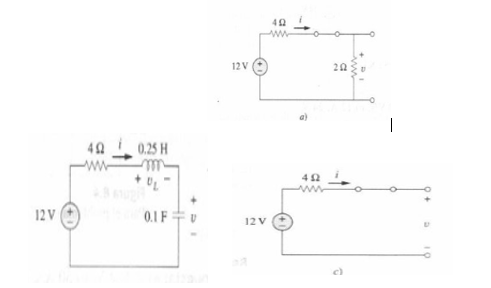
\includegraphics[width=0.9\linewidth]{ultimocirc}
\end{center}
Circuito equivalente para:
$t(0^{-})$
$t(^{+})$
$t\longrightarrow \infty$

Dado que la corriente del inductor y la tensión del capacitor no pueden cambiar abruptamente, 
$i(0^{+} )=i(0^{-} )=2A$,           $v(0^{+} )=v(0^{-} )=4V$

	En $t=0^{+}$, el interruptor está abierto;t anto por el inductor como por el capacitor fluye la misma corriente. Así.
	
$$i_c (0^+ )=i(0^+ )=2A$$

Puesto que:
$$c\frac{dv}{dt}=ic, \frac{dv}{dt}=\frac{ic}{c} y \frac{dv(0^{+})}{dt}=\frac{ic(0^{+})}{c}=\frac{2}{0.1}=20 \frac{v}{s}$$


De igual manera, como $Ldi⁄dt=v_l,di⁄dt=v_l⁄L$,ahora se obtine $v_l$ aplicando la LTK, el resultado será:

$$-12+4_i(0^{+})+v_l(0^{+})+v(0^{+})=0$$

Es decir,

$$v_L(0^{+})=12-0-4=0$$

En consecuencia:

$$\frac{di(0^{+})}{dt}=\frac{v_L(0^{+})}{L}=\frac{0}{0.25}=0 \frac{A}{s}$$

	Para $t>0$, el circuito pasa por un transiente. Pero como $t\longrightarrow\infty$, llega otra vez al estado estable. El inductor actúa como cortocircuito y el capacitor como circuito abierto, de modo que el circuito de b) se convierte en el que aparece en c), del que se tiene $i(\infty)=0 A$,  $V(\infty)=12 V$
\chapter{Ejercicios de aplicaciones}
1. 	Un bloque de 5 kg. de masa se mueve entre guías verticales suspendido por dos muelles iguales de constante recuperadora elástica $ K1 = K2$ = 60 N/m, como se indica en la figura. Calcular:
\begin{center}
	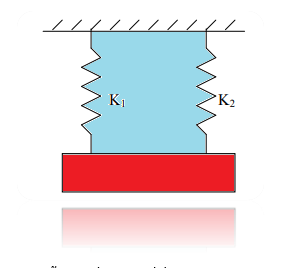
\includegraphics[width=0.5\linewidth]{EJERCICIO1}
\end{center}
a)	Ecuación de las pequeñas oscilaciones del sistema

\textbf{\begin{center}
		SOLUCION:
\end{center}}
Los muelles están asociados en paralelo y oscilan con vibración libre sin amortiguamiento de acuerdo a la ecuación:
\begin{equation}
	mx''+k_px=0
\end{equation}

La ecuación de  vibración  libre sin amortiguamiento, procedemos identificar los elementos de la ecuación. 

masa$\to m=5kg$
\begin{equation}
	k_p=k_1+k_2=60+60=120 \frac{N}{m}
\end{equation}
Luego la ecuación diferencial de segundo orden es:

\begin{equation}
	5x''+120x=0\leftrightarrow x''+24x=0
\end{equation}
Luego, usando la ecuación auxiliar se tiene que resolver la ecuación siguiente:

$$r^{2}+24=0$$
El cual por un proceso algebraico podemos deducir que:
$r^{2}=-24$

\begin{center}
	$r_1=\sqrt{-24}, \longrightarrow r_2=-\sqrt{-24}$
\end{center}
es decir
\begin{center}
	$r_1=2\sqrt{6i}, \longrightarrow r=-2\sqrt{6i}$
\end{center}

Ahora bien para dos  raíces complejas diferentes se tiene que  la solución es de la forma:

\begin{equation}
	x=e^{at}(C_1\cos(\beta t)+C_2 sin(\beta t))
\end{equation}

Note que   a=0 , pues corresponde a la parte real la cual es nula, dado que solo existe la parte compleja  dada por símbolo $ \beta$

\begin{equation}
	x=e^{0}(C_1 \cos(2\sqrt{6t})+ C_2 sin(2\sqrt{6t})) ,\hspace{0.3cm} \text{Obsevemos que}: e^{0}=1
\end{equation}
		\begin{equation}
x=(C_1 \cos(2\sqrt{6t})+ C_2 sen(2\sqrt{6t}))
					\end{equation}
\begin{equation}
	x=(Asen(2\sqrt{6t}+\varphi))
\end{equation}

Además si tenemos el dato de:

$F=10 sen(t)$

Luego se tiene la ecuación de una vibración forzada sin amortiguamiento 
\begin{equation}
	mx¨+k_px=F
\end{equation}
\begin{equation}
	5x¨+120x=10 sen(t)\leftrightarrow x¨+24x=2sen(t)
\end{equation}

Cuya solución es: 
\begin{equation}
	x=(C_1 \cos(2\sqrt{6t})+C_2 sen(2\sqrt{6t}))+\frac{2}{23} sen(t)
\end{equation}
La ecuación particular se puede determinar de manera ''fácil''  usando variación de parámetro, el cual por no alargar más el tema no se ha explicado en este documento.
\newpage
2) El sistema de la figura consta de una masa, dos muelles  un amortiguador de caracteristicas:

\begin{center}
	$m=30kg; \hspace{0.3cm}k_1=60 \frac{N}{m};\hspace{0.3cm} k_2=90 \frac{N}{m};\hspace{0.3cm} C=90 N.\frac{s}{m}$
\end{center}

ED del movimiento y su solución general

\begin{center}
	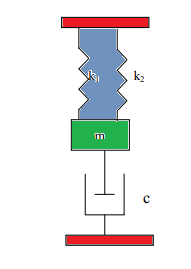
\includegraphics[width=0.4\linewidth]{EJERCIIO2}
\end{center}

\begin{center}
	\textbf{Solución:}
\end{center}

a)	La ecuación diferencial del movimiento de una vibración libre amortiguada es:
\begin{equation}
	mx¨+cx´+k_px=0
\end{equation}

Solución:
a)	La ecuación diferencial del movimiento de una vibración libre amortiguada es:
$m=30kg; k_1=60 \frac{N}{m}; k_2=90 \frac{N}{m}; C=90 N.\frac{s}{m}$
Luego la ecuación diferencial de segundo orden es:
\begin{equation}
	30x¨+90x´+150x=0\leftrightarrow x¨+3x´+5x=0
\end{equation}
Luego, como el ejercicio anterior usando la ecuación auxiliar se tiene que,

$r^{2}+3r+5=0$
una forma rapida, de resolver la anterior ecuación es usando la formula cuadrática, esto  para encontrar las raíces  donde; $a=1$, $b=3$, y $c=5$
$$\begin{array}{ccc}
	r&=&\frac{-b\pm(\sqrt{b^{2})-4ac}}{2a}\\
	r&=&\frac{-3\pm(\sqrt{3^{2}-4*1*5})}{2*1}\\
	r&=&\frac{-3\pm(\sqrt{9-20})}{2}\\
\end{array}$$
luego,
$$r_1=\frac{-3+(\sqrt{11i})}{2}=-\frac{3}{2}-\frac{\sqrt{11i}}{2}$$
y la otra raíz
$$r_2=\frac{-3+(\sqrt{11i})}{2}=-\frac{3}{2}-\frac{\sqrt{11i}}{2}$$

Ahora bien para dos  raíces complejas diferentes se tiene que  la solución es de la forma:

$$x=e^{at}\left( C_1 \cos(\beta t)\right) +C_2 sen\left( \beta t\right) $$

Note que   $a=-3/2$  , pues corresponde a la parte real la cual es  no nula,  po otro lado  la parte compleja  dada por símbolo  $\beta$

\begin{equation}
	x=e^{-\frac{3t}{2}}\left( C_1\cos\left( \frac{\sqrt{11i}}{2}t\right) +C_2 sen\left( \frac{\sqrt{11i}}{2}t\right) \right) 
\end{equation}

\begin{equation}
	x=\left( e^{-\frac{3t}{2} (sen(\frac{\sqrt{11i}}{2}t) )+\varphi}\right) 
\end{equation}
	
Además si tenemos el dato de:
 $F=30 sen(t)$

Luego se tiene la ecuación de una vibración forzada con  amortiguamiento 
\begin{equation}
	mx''+cx'+k_px=F
\end{equation}
\begin{equation}
	30x''+90x'+150x=30sen(t)\leftrightarrow x''+3x'+5x=sen(t)
\end{equation}
Cuya solución es:
\begin{equation}
	x=e^{-\frac{3b}{2}}\left( C_1\cos\left( \frac{\sqrt{11i}}{2}t\right) +C_2 sen\left( \frac{\sqrt{11i}}{2}t\right) +\frac{4}{25}sen(t)*\frac{3}{25)\cos(t)}\right) 
\end{equation}
\newpage
\thispagestyle{empty}\bigskip
\begin{center}\rule{0.9\textwidth}{0.1mm} \end{center}
{\sf
	\begin{center}
		\Large \textsc{Bibliografía}%
	\end{center}
}\bigskip
{\small \begin{itemize}
	\item https://dokumen.tips/documents/capitulo-08-circuitos-de-segundo-orden-563de7f5e06f6.html?page=8
	\item https://ocw.unican.es/pluginfile.php/1301/course/section/15 94/12-Oscilaciones.pdf
	\item https://es.slideshare.net/WillianDiaz1/edo-circuitos- electricos.
	\item 	http://canek.uam.mx/Ecuaciones/Teoria/5.AplicacionesOrde nSuperior/ImpRLCContinua.pdf
	\item http://canek.uam.mx/Ecuaciones/Teoria/5.AplicacionesOrde nSuperior/ImpArmonicoSimple.pdf.
	\item Dennis G.text Zill \textbf{Ecuaciones Diferenciales} 
	\item Shephy L. Ross \textbf{Ecuaciones Diferenciales}
\end{itemize}
}
\end{document}

